%!TEX root = main.tex

\section{Decision procedure for $\strline_{\sf reg}$} \label{sec:decision}

In this section, we shall prove Theorem~\ref{thm-main}.
%
%\begin{theorem}\label{thm-main}
%The path feasibility of $\strline_{\sf reg}$ is decidable.
%\end{theorem}
%
We first show that both $\extract$ and $\replaceall$ functions can be transformed into PSST, then compute the pre-images of regular languages under PSSTs and remove all the assignment statements, finally solve the nonemptiness of intersection of regular languages. The aforementioned procedure extends the approach of backward reasoning proposed in \cite{CCH+18,CHL+19} in the following sense: While \cite{CCH+18,CHL+19} used the standard one-way and two-way transducers, we introduce PSST, a new transducer model $\extract$ and $\replaceall$, where priorities are used to model the greedy and non-greedy semantics of capturing groups and string variables are used to model the back references. Moreover, as we have shown in Theorem~\ref{theorem:psst_preimage}, the pre-images of regular languages under PSSTs are still regular and can be computed effectively.

In the sequel, we shall show that semantically equivalent PSSTs can be effectively constructed from the $\extract$ and $\replaceall$ functions. 

\begin{lemma}\label{lem-extract}
From $\extract_{i,e}(x)$, a PSST $\cT_{\extract_{i,e}}$ can be constructed such that $\cR_{\cT_{\extract_{i,e}}} = \{(w, w') \mid w'= \extract_{i,e}(w)\}$.
\end{lemma}

\begin{lemma}\label{lem-replace}
From $\replaceall_{\pat, \rep}(x)$, a PSST $\cT_{\replaceall_{\pat, \rep}}$ can be constructed such that $\cR_{\cT_{\replaceall_{\pat, \rep}}} = \{(w, w') \mid w'= \replaceall_{\pat, \rep}(w)\}$.
\end{lemma}

With Lemma~\ref{lem-extract}-\ref{lem-replace}, the path feasibility of $\strline_{\sf reg}$ is reduced to the path feasibility of string-manipulating programs that are a sequential composition of the statements of the form $z:=x \concat y$, $y:=\cT(x)$ and $\ASSERT{x \in \cA}$, where $\cT$ is a PSST and $\cA$ is an FA. Let us use  $\strline'_{\sf reg}$ to denote the class of such programs. Then we can follow the backward reasoning approach of the OSTRICH solver proposed in \cite{CCH+18,CHL+19} and solve the path feasibility of $\strline'_{\sf reg}$ by repeating the following procedure, until no more assignment statements are left:\\
Let $S$ be the current $\strline'_{\sf reg}$ program.
\begin{itemize}
\item If the last assignment statement of $S$ is $y:=\cT(x)$, then let $\ASSERT{y \in \cA_1}, \cdots, \ASSERT{y \in \cA_n}$ be an enumeration of all the assertion statements for $y$ in $S$. Compute $\cR^{-1}_\cT(\Lang(\cA_1))$ as an FA $\cB_1$, $\cdots$, and $\cR^{-1}_\cT(\Lang(\cA_n))$ as $\cB_n$. Remove  the assignment  $y:=\cT(x)$ and add the assertion statements $\ASSERT{x \in \cB_1}$; $\cdots$; $\ASSERT{x \in \cB_n}$. 
%
\item If the last assignment statement of $S$ is $z:=x \concat y$, then let $\ASSERT{z \in \cA_1}, \cdots, \ASSERT{z \in \cA_n}$ be an enumeration of all the assertion statements for $z$ in $S$. Compute $\concat^{-1}(\Lang(\cA_1))$, the pre-image of $\concat$ under $\Lang(\cA_1)$, as a collection of FA pairs $(\cB_{1,j}, \cC_{1,j})_{j \in [m_1]}$, $\cdots$, and $\concat^{-1}(\Lang(\cA_n))$ as $(\cB_{n, j}, \cC_{n,j})_{j \in [m_n]}$ (c.f. \cite{CHL+19}). Remove the assignment $z:=x \concat y$, nondeterministically choose the indices $j_1 \in [m_1], \cdots, j_n \in [m_n]$, and add the assertion statements $\ASSERT{x \in \cB_{1,j_1}}; \ASSERT{y \in \cC_{1, j_1}}$; $\cdots$; $\ASSERT{x \in \cB_{n,j_n}}; \ASSERT{y \in \cC_{n, j_n}}$. 
\end{itemize}

It remains to show Lemma~\ref{lem-extract} and Lemma~\ref{lem-replace}. As a warm-up, we first present a cornerstone of the proof of the two lemmas, namely, the construction of PFAs from $\regexp[\sf CG]$ expressions, which is adapted from the pNFA construction in \cite{BDM14}, which in turn is a variant of the standard
Thompson construction \cite{Thompson68}. 
%We include the construction here for improving the readability.  
Afterwards, we prove the two lemmas. 


\subsection{From $\regexp[\sf CG]$ to PFA}
\label{construction:pnfa}

%\begin{figure*}
%	\centering
%	\includegraphics{pglushkov_01}
%	\caption{pNFA $A_e$ for (a) $e=e_1+e_2$ (b) $e=e_1^{\ast}$ and (c) $e=e_1 \concat e_2$ where $\varepsilon \in \Lang(e_1)$ and $\varepsilon \notin \Lang(e_2)$. A transition of lower priority is depicted thiner and more densely dotted. }
%	\label{fig:pglushkov}
%\end{figure*}

For any $e \in \regexp[\sf CG]$, a PFA $\cA_e$ is constructed recursively in the sequel. The constructed PFA $\cA_e$ satisfies that it has a unique initial state and a unique final state  without outgoing transitions.
%The original construction on regular expressions
%produces an FA without $\varepsilon$-transitions, which we denote by $G_e$.
%We refer the reader to \cite{Gluskov61} for 
%details of how to construct $G_e$. %\tl{is this just the textbook construction?}
%
%The pNFA $A_e$ is obtained by recursively adding priority to $G_e$ as follows:
\begin{itemize}
\item If $e =\emptyset$, then $\cA_e = (\{q_0,f_0\}, \Sigma, \delta, \tau, q_0, f_0)$, where $\delta(q_0, \sigma) = \delta(f_0, \sigma) = ()$ for every $\sigma \in \Sigma$, $\tau(q_0) = \tau(f_0)= ((); ())$.

  \item If $e = \varepsilon$, then  $\cA_e = (\{q_0, f_0\}, \Sigma, \delta, \tau, q_0, f_0)$, where  $\delta(q_0, \sigma) = \delta(f_0, \sigma) = ()$ for every $\sigma \in \Sigma$, $\tau(q_0) = ((f_0); ())$, and $\tau(f_0) = ((); ())$. 

  \item If $e = a$, then $\cA_e = (\{q_0, f_0\}, \Sigma, \delta, \tau, q_0, f_0)$, where  $\delta(q_0, a) = (f_0)$, $\delta(q_0, \sigma) = ()$ for every $\sigma \in \Sigma \setminus \{a\}$, $\tau(q_0) = ((); ())$, and $\tau(f_0) = ((); ())$.
    
  \item If $e = (e_1)$, then $\cA_e = \cA_{e_1}$.
  
  \item If $e = e_1 + e_2$, and suppose $\cA_{e_1} = (Q_1,
  \Sigma, \delta_1, \tau_1, q_1, f_1)$ and $\cA_{e_2} = (Q_2, \Sigma,
  \delta_2, \tau_2, q_2, f_2)$, then $\cA_e = (Q_1 \cup Q_2 \cup \{q_0, f_0\}, \Sigma,
  \delta, \tau, q_0, f_0)$, where  
  \begin{itemize}
 \item $q_0, f_0 \not \in Q_1 \cup Q_2$, 
 \item $\delta(q) = \delta_i(q)$ for every $q \in Q_i$ ($i=1,2$), 
$\delta(q_0, \sigma) = \delta(f_0, \sigma) = ()$ for every $\sigma \in \Sigma$, 
%
 \item $\tau(q) = \tau_i(q)$ for every $q \in Q_i$ ($i =1,2$), $\tau(q_0) = ((q_1,q_2); ())$,  $\tau(f_1) = \tau(f_2) = ((f_0); ())$, and $\tau(f_0) = ((); ())$.
 \end{itemize}
%
  \item If $e = e_1 \concat e_2$, and suppose $\cA_{e_1} = (Q_1,
  \Sigma, \delta_1, \tau_1, q_1, f_1)$ and $\cA_{e_2} = (Q_2, \Sigma,
  \delta_2, \tau_2, q_2, f_2)$, then $\cA_e = ( Q_1 \cup Q_2, \Sigma, \delta, \tau, q_1,
  f_2)$, where 
  \begin{itemize}
    \item for every $q \in Q_i$, $\delta(q) = \delta_i(q)$ ($i = 1,2$),
    
    \item for every $q \in Q_2$, $\tau(q) = \tau_2(q)$, 
%
    \item for every $q \in Q_1 \setminus \{f_1\}$, $\tau(q) = \tau_1(q)$, and $\tau(f_1) = ((q_2); ())$.
  \end{itemize}
%  
  \item If $e = e_1^{\ast}$, and suppose  $\cA_{e_1} = (Q_1,
  \Sigma, \delta_1, \tau_1, q_1, f_1)$, then $\cA_e = (Q_1 \cup \{f_0\}, \Sigma,
  \delta, \tau, q_1, f_0)$, where 
  \begin{itemize}
  \item $f_0 \not \in Q_1$,
  
    \item for every $q \in Q_1$ and $\sigma \in \Sigma$, $\delta(q, \sigma) = \delta_1(q, \sigma)$, 
    %moreover, $\delta(q_0, \sigma) = \delta(f_0, \sigma)  = ()$,
    
    \item for every $q \in Q_1 \setminus \{q_1, f_1\}$,  $\tau(q) = \tau_1(q)$, moreover, $\tau(q_1) = (\pi_1(\tau_1(q_1)); (\pi_2(\tau_1(q_1)), f_0))$, $\tau(f_1) = ((q_1); ())$, and $\tau(f_0) = ((); ())$. (Intuitively, the $\varepsilon$-transitions from $f_1$ to $q_1$ and from $q_1$ to $f_0$ respectively are added, moreover, the $\varepsilon$-transition from $q_1$ to $f_0$ is of the lowest priority.)
  \end{itemize}
 %
  \item If $e = e_1^{\ast?}$, and suppose $\cA_{e_1} = (Q_1,
  \Sigma, \delta_1, \tau_1, q_1, f_1)$, then $\cA_e = (Q_1 \cup \{f_0\}, \Sigma,
  \delta, \tau, q_1, f_0)$, where 
  \begin{itemize}
  \item $q_0, f_0 \not \in Q_1$,
  
    \item for every $q \in Q_1$ and $\sigma \in \Sigma$, $\delta(q, \sigma) = \delta_1(q, \sigma)$, 
    %moreover, $\delta(q_0, \sigma) = \delta(f_0, \sigma)  = ()$,
    
    \item for every $q \in Q_1 \setminus \{q_1, f_1\}$,  $\tau(q) = \tau_1(q)$, moreover, $\tau(q_1) = ((f_0, \pi_1(\tau_1(q_1))); \pi_2(\tau_1(q_1)))$, $\tau(f_1) = ((q_1); ())$, and $\tau(f_0) = ((); ())$. (The $\varepsilon$-transition from $q_1$ to $f_0$ is of the highest priority.)
  \end{itemize}  
\end{itemize}

%The key transitions of some non-trivial cases of the construction are illustrated in Figure.\ref{fig:pglushkov}.

% An important property of the automaton $G_e$ and thus $A_e$ is that, for any subexpression $e'$ of $e$, there must be a subgraph of $A_{e}$ corresponding to $e'$. We denote this subgraph by $A_{e}[e']$. This subgraph can be seen as the automaton obtained by removing from $A_{e'}$ the state $q_0$ and all transitions from it.

\begin{example}
Let $e_1 = a^\ast$ and $e_2 = a^{\ast ?}$. Then the PFAs $\cA_{e_1} = (Q_1, \Sigma, \delta_1, \tau_1, q_0, q_3)$ and $\cA_{e_2} =  (Q_2, \Sigma, \delta_2, \tau_2, q_0, q_3)$ are illustrated in Figure~\ref{fig-retopfa}: (i), (ii), where thicker solid lines (resp. dashed lines) denote the $\varepsilon$-transitions of higher (resp. lower) priorities than non-$\varepsilon$-transitions. For instance, in $\cA_{e_1}$, $\tau_1(q_0) = ((); (q_2))$ and $\tau_1(q_1) = ((q_0); ())$, while in $\cA_{e_2}$, $\tau_2(q_0) = ((q_2); ())$ and $\tau_2(q_1) = ((q_0); ())$. Note that $\cA_{e_1}$ and $\cA_{e_2}$ are slightly different from those in Example~\ref{exmp-pfa}.
\begin{figure}[ht]
\centering
%\rule{\linewidth}{0cm}
\includegraphics[scale=0.8]{retopfa.pdf}
\caption{$\cA_{e_1}$ and $\cA_{e_2}$ for $e_1= a^\ast$ and $e_2 = a^{\ast?}$}
\label{fig-retopfa}
\end{figure}
\end{example}
 
%For instance, if $e = (a (ab)^*)^*$ and $e' = a(ab)^*$, then $A_{e}[e']$ is the subgraph of $A_{e}$ comprising the states $\{a_1, a_2, b_3\}$ and the transitions $\{(a_1, a, a_2), (a_2, b, b_3), (b_3, a, a_2)\}$.
 
%Figure.\ref{fig:pglushkov} also illustrates the subgraphs corresponding to direct subexpressions of $e$.


%\begin{definition}
%Let $e \in \regexp[\sf CG]$ and $e'$ be a subexpression of $e$. Then a copy of $\cA_{e'}$ in $\cA_e = (Q, \Sigma, \delta, \tau, q_0, f_0)$ is a PFA $(Q', \Sigma, \delta', \tau', q'_0, f'_0)$ such that  
%\begin{itemize}
%\item $Q' \subseteq Q$, $q'_0, f'_0 \in Q'$, 
%\item $\delta'$ is the restriction of $\delta$ to $Q'$, with the outgoing transitions of $f'_0$ removed, specifically, for every $\sigma \in \Sigma$ and $q \in Q' \setminus \{f'_0\}$, $\delta'(q, \sigma) = \delta(q, \sigma)$, $\tau'(q) = \tau(q)$, $\delta'(f'_0, \sigma) = ()$, and $\tau'(f'_0) = ((); ())$,
%\item $(Q', \Sigma, \delta', \tau', q'_0, f'_0)$ is isomorphic to $\cA_{e'}$.
%\end{itemize}
%\end{definition}

From the aforementioned recursive construction of $\cA_e$, we know that for each subexpression $e'$ of $e$, a PFA for $e'$, which is isomorphic to $\cA_{e'}$, is also constructed. Let us use ${\sf Sub}_{e'}[\cA_e]$ to denote this PFA for $e'$, which, roughly speaking, is a subgraph of $\cA_e$.
%\begin{proposition}\label{prop-subexp}
%Let $e \in \regexp[\sf CG]$. Then for every subexpression $e'$ of $e$, there is a unique copy of $\cA_{e'}$ in $\cA_e$, denoted by ${\sf Sub}_{e'}[\cA_e]$.
%\end{proposition}

%\begin{definition}
%  Let $A_e$ be the pNFA constructed for $e$, and $p = q_0 \sigma_1 q_1 \ldots
%  \sigma_m q_m$ is the accepting run of $A_e$ on string w. For any subexpression $e'$ of $e$, we say a
%  consecutive sequence of states $q_i q_{i + 1} \ldots q_{j - 1} q_j$ in p is
%  a maximal $e'$-match, if $q_i \in \tmop{Start} (e')$, $q_j \in \tmop{End}
%  (e')$, $(q_{i - 1}, \sigma_i, q_i)$ is not a transition in $A_e [e']$, and
%  for any $k \in [i, j]$, $q_k$ is a vertex in $A_e [e']$. Moreover, if $j
%  \neq m$, then $(q_j, \sigma_{j + 1}, q_{j + 1})$ is not a transition in $A_e
%  [e']$.
  
%  We use $p_{e', e} (w)$ to denote the sequence of disjoint maximal $e'$-match
%  $w_1 \ldots w_n$, in the order they occur in p. Note that in $A_e$, all
%  states except $q_0$ are labeled by a letter, thus a maximal $e'$-match can
%  be seen as a string.
%\end{definition}

%The following  theorem states the equivalence of the accepting match of a \regexp[\sf CG] $e$ and the accepting run of $A_e$ on the same input string, thus the construction precisely captures the semantics. % in \ref{semantics:regex}.
%\begin{theorem}
% \label{theorem:regex_pnfa_equiv}
%  For any regular expression e, subexpression $e'$ of e, and $w \in L (e)$,
%  $m_{e', e} (w) = p_{e', e} (w)$
%\end{theorem}
%
%For simplicity, we refer the reader to the appendix for proof.


 
\subsection{Proof of Lemma~\ref{lem-extract}-\ref{lem-replace}}

We first prove Lemma~\ref{lem-extract}, namely, show how to construct a PPST $\cT_{\extract_{i,e}}$ for $\extract_{i,e}$.

\paragraph*{Construction of $\cT_{\extract_{i,e}}$.} 
Let $e'$ be the subexpression corresponding to the $i$-th capturing group of $e$. In particular, if $i=0$, then $e' = e$. 

Suppose $\cA_e = (Q, \Sigma, \delta, \tau, q_0, f_0)$. Then $\cT_{\extract_{i,e}}$ is obtained from $\cA_e$ by adding two fresh states $q'_0, f'_0$ such that (see Figure~\ref{fig-psst-extract})
\begin{itemize}
\item $\cT_{\extract_{i,e}}$ goes from $q'_0$ to $q_0$ via an $\varepsilon$-transition of higher priority than the non-$\varepsilon$-transitions, in order to search for the first match of $e$, 
%
\item then $\cT_{\extract_{i,e}}$ simulates $\cA_e$ and stores the match of the $i$-th capturing group of $e$ into a string variable $x$,  
%
\item when the first match of $e$ is found, $\cT_{\extract_{i,e}}$ goes from $f_0$ to $f'_0$ via an $\varepsilon$-transition, then keeps idle, and finally output the content of $x$.
\end{itemize}

\begin{figure}[ht]
\centering
%\rule{\linewidth}{0cm}
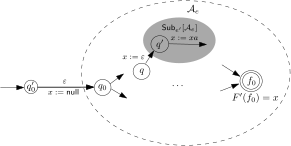
\includegraphics[scale=0.8]{psst-extract.pdf}
\caption{The PSST for $\extract_{i,e}$}
\label{fig-psst-extract}
\end{figure}

Formally, $\cT_{\extract_{i,e}} = (Q \cup \{q'_0, f'_0\}, \Sigma, X, \delta', \tau', E, q'_0, F)$ where 
\begin{itemize}
\item $q'_0, f'_0 \not \in Q$,

\item  $X = \{x\}$,
%
\item $F(f'_0) = x$, and $F(q')$ is undefined for every $q' \in Q \cup \{q'_0\}$,

\item $\delta'$ and $\tau'$ are obtained from $\delta$ and $\tau$ as follows,
\begin{itemize}
\item $\delta'(q'_0, \sigma) = (q'_0)$ for every $\sigma \in \Sigma$, and $\tau'(q'_0) = ((q_0); ())$,
%
\item  for every $q \in Q \setminus \{f_0\}$ and $\sigma \in \Sigma$, $\delta'(q, \sigma) = \delta(q, \sigma)$ and $\tau'(q) = \tau(q)$, 
%
\item $\delta'(f_0, \sigma) = ()$ for every $\sigma \in \Sigma$ and $\tau'(f_0) = ((f'_0); ())$,
%
\item $\delta'(f'_0, \sigma) = (f'_0)$ for every $\sigma \in \Sigma$ and $\tau'(f'_0) = ((); ())$,
\end{itemize}
%
\item $E$ is defined as follows, 
\begin{itemize}
\item for every transition $(q, \sigma, q')$ with  $\sigma \in \Sigma^\varepsilon$ in ${\sf Sub}_{e'}[\cA_e]$, we have $E(q, \sigma, q')(x) = x\sigma$.
\item for all the other transitions $(q, \sigma, q')$ with $\sigma \in \Sigma^\varepsilon$ in $\cT_{\extract_{i,e}}$, we have $E(q, \sigma, q')(x) = x$
\end{itemize}
%
\end{itemize}

\tl{tbc}


\paragraph*{Construction of $\cT_{\replaceall_{\pat, \rep}}$.} 
Let $\$i_1, \cdots, \$i_k$ with $i_1 < \cdots < i_k$ be an enumeration of all the references in $\rep$. 
Moreover, for every $j \in [k]$, let $e'_{i_j}$ be the subexpression of $\pat$ corresponding to the $i_j$-th capturing group.

Suppose $\cA_\pat = (Q, \Sigma, \delta, \tau, q_0, f_0)$. Then $\cT_{\replace_{\pat,\rep}}$ is obtained from $\cA_\pat$ by adding a fresh states $q'_0$ such that (see Figure~\ref{fig-psst-replace})
\begin{itemize}
\item $\cT_{\replace_{\pat,\rep}}$ goes from $q'_0$ to $q_0$ via an $\varepsilon$-transition of higher priority than the non-$\varepsilon$-transitions, in order to search the first match of $\pat$ starting from the current position, 
%
\item when $\cT_{\replace_{\pat,\rep}}$ stays at $q'_0$, it keeps appending the current letter to the end of $x_0$, 
%
\item starting from $q_0$, $\cT_{\replace_{\pat,\rep}}$ simulates $\cA_\pat$ and stores the matches of the $\$i_1$-th, $\ldots$, $\$i_k$-th capturing groups of $\pat$ into the string variables $x_1, \cdots, x_k$ respectively,   
%
\item when the first match of $\pat$ is found, $\cT_{\replace_{\pat,\rep}}$ goes from $f_0$ to $q'_0$ via an $\varepsilon$-transition, appends the current replacement string, which is $\rep[x_1/\$_{i_1}, \cdots, x_k/\$_{i_k}]$, to the end of $x_0$, and keeps searching for the next match of $\pat$, 
\end{itemize}

\begin{figure}[ht]
\centering
%\rule{\linewidth}{0cm}
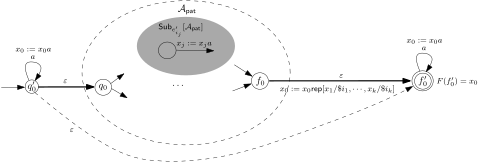
\includegraphics[scale=0.65]{psst-replace.pdf}
\caption{The PSST for $\replace_{\pat,\rep}$}
\label{fig-psst-replace}
\end{figure}

Formally, $\cT_{\replaceall_{\pat, \rep}} =$ $(Q \cup \{q'_0\}$, $\Sigma$, $X$, $\delta'$, $\tau', E, q'_0, F)$ where
\begin{itemize}
\item $q'_0 \not \in Q$,

\item  $X = \{x_0, x_1, \cdots, x_k\}$,
%
\item $F(q'_0) = x_0$, and $F(q')$ is undefined for every $q' \in Q$,
%
\item $\delta'$ and $\tau'$ are obtained from $\delta$ and $\tau$ as follows,
\begin{itemize}
\item $\delta'(q'_0, \sigma) = (q'_0)$ for every $\sigma \in \Sigma$, and $\tau'(q'_0) = ((q_0); ())$,
%
\item for every $q \in Q \setminus \{f_0\}$ and $\sigma \in \Sigma$, $\delta'(q, \sigma) = \delta(q, \sigma)$ and $\tau'(q) = \tau(q)$, 
%
\item $\delta'(f_0, \sigma) = ()$ for every $\sigma \in \Sigma$ and $\tau'(f_0) = ((q'_0); ())$,
\end{itemize}
%
\item $E$ is defined as follows, 
\begin{itemize}
\item for every transition $(q, \sigma, q')$ with $\sigma \in \Sigma^\varepsilon$ in $\cA_\pat$, $E(q, \sigma, q')(x_0) = x_0$,
%
\item for every transition $(q, \sigma, q')$ with $\sigma \in \Sigma^\varepsilon$ and every $j \in [k]$,  if $(q, \sigma, q')$ occurs in ${\sf Sub}_{e'_{i_j}}[\cA_\pat]$, then $E(q, \sigma, q')(x_j) = x_j\sigma$, otherwise, $E(q, \sigma, q')(x_j) = x_j$,
%
%\item for all the other transitions $(q, \sigma, q')$ with $\sigma \in \Sigma^\varepsilon$ in $\cA_e$, we have $E(q, \sigma, q')(x) = x$, 
%
\item  for every $\sigma \in \Sigma$, $E(q'_0, \sigma, q'_0)(x_0) = x_0\sigma$, and for every $j \in [k]$, $E(q'_0, \sigma, q'_0)(x_j) = x_j$, 

\item $E(q'_0, \varepsilon, q_0)(x_j) = x_j$ for every $j \in [k] \cup \{0\}$, 
%
\item $E(f_0, \varepsilon, q'_0)(x_0) = x_0 \rep[x_1/\$i_1,\ldots, x_k/\$i_k]$, and for every $j \in [k]$, $E(f_0, \varepsilon, q'_0)(x_j) = \varepsilon$, 

\end{itemize}
%
\end{itemize}


\begin{definition}[Pre-image]
For a string relation $R \subseteq \Sigma^* \times \Sigma^*$ and $L \subseteq \Sigma^*$, we define the \emph{pre-image} of $L$ under $R$ as $R^{-1}(L):=\{w \in \Sigma^* \mid \exists w'.\ w' \in L \mbox{ and } (w, w') \in R\}$. 
\end{definition}
 
\begin{theorem}[Pre-image of \PSST{}]
  \label{theorem:psst_preimage}
  Given a \PSST{} $\psst = (Q_T, \Sigma$, $X, \delta_T, \tau_T, E_T,  q_{0, T}, F_T)$ and an \FA{} $\Aut
  = (Q_A, \Sigma, \delta_A, q_{0, A}, F_A)$, we can compute an \FA{} $\cB = (Q_B,
  \Sigma, \delta_B, q_{0, B}, F_B)$ in exponential time  such that $\Lang(\cB) = \cR^{-1}_{\cT}(\Lang(\Aut))$.
\end{theorem}

\tl{another way is to first define B as a PFA, could make the construction a bit modular?}\zhilin{Add a counter example for this natural idea.}
 
Let $\psst = (Q_T, \Sigma$, $X, \delta_T, \tau_T, E_T,  q_{0, T}, F_T)$ be a \PSST{}  and $\Aut
  = (Q_A, \Sigma, \delta_A, q_{0, A}, F_A)$ be an \FA{}. Without loss of generality, we assume that $\Aut$ contains no $\varepsilon$-transitions. 

To illustrate the intuition of the FA construction, let us start with the following natural idea of firstly constructing a PFA $\cB$ for the pre-image: $\cB$ simulates the run of $\psst$ on $w$, and, for each $x \in X$, records an $\Aut$-abstraction of the string stored in $x$, that is, the set of state pairs $(p, q) \in Q_A \times Q_A$ such that starting from $p$, $\Aut$ can reach $q$ after reading the string stored in $x$. Specifically, the states of $\cB$ are of the form $(q, \rho)$ with $q \in Q$ and $\rho \in (\cP(Q_A \times Q_A ))^{X}$. Moreover, the priorities of $\cB$ inherit those of $\Aut$. The PFA $\cB$ is then transformed to an equivalent FA by simply dropping all priorities. We refer to this FA as $\cB'$.

Nevertheless, it turns out that this construction method is flawed: A string $w$ is in $\cR^{-1}_{\cT}(\Lang(\Aut))$ iff the (unique) accepting run of $\cT$ on $w$ produces an output $w'$ that is accepted by $\Aut$. However, a string $w$ is accepted by $\cB'$ iff there is a run of $\cT$ on $w$, not necessarily of the highest priority, producing an output $w'$ that is accepted by $\Aut$. The following example illustrates the flaw of the construction above.

\begin{example}
\label{pre-image-count-examp}
Let $\cT$ be the PSST and $\cA$ be the FA in Figure~\ref{fig-pre-image-count-exmp}, that is, 
\begin{itemize}
\item $\cT=(\{q_0, q_1, q_2\}, \{a,b,c\}, \{x_0\}, \delta_T, \tau_T, E_T, q_0, F_T)$, where $\delta_T(q_0, \sigma) = (q_0)$, $\delta_T(q_1, a) = (q_1)$, $\delta_T(q_2, \sigma) = (q_2)$, $\tau_T(q_0) = ((q_1); ())$, $\tau_T(q_1)=((q_0, q_2);())$, and $\tau_T(q_2)= ((); ())$, $E_T(q_0, \sigma, q_0) (x_0) = x_0 \sigma$, $E_T(q_1, \varepsilon, q_0) (x_0) = x_0 c$, $E_T(q_1, \varepsilon, q_2) (x_0) = x_0 c$, $E_T(q_2, \sigma, q_2) (x_0) = x_0 \sigma$, for $\sigma \in\{ a, b\}$. Moreover, $F_T(q_2)= x_0$;
%
\item $\cA = (\{p_0\}, \{a,b,c\}, \delta_A, p_0, \{p_0\})$, where $\delta_A$ = $\{(p_0, \sigma, p_0)$ $\mid \sigma = b, c\}$.
\end{itemize}

Let us consider $w = a$. The accepting run of $\cT$ on $w$ is $q_0 \xrightarrow{\varepsilon} q_1 \xrightarrow[x_0:=x_0c]{\varepsilon} q_0 \xrightarrow[x_0:=x_0a]{a} q_0 \xrightarrow{\varepsilon} q_1 \xrightarrow[x_0:=x_0c]{\varepsilon} q_2$, producing an output $cac \not \in \Lang(\cA)$. Therefore, $a \not \in \cR_\cT^{-1}(\Lang(\cA))$. Nevertheless, if we consider the FA $\cB'$ constructed from $\cT$ and $\cA$,  it turns out that $\cB'$ does accept $w$, witnessed by the run $(q_0, \{(p_0,p_0)\}) \xrightarrow{\varepsilon} (q_1, \{(p_0,p_0)\}) \xrightarrow{a} (q_1, \{(p_0, p_0)\}) \xrightarrow{\varepsilon}  (q_2, \{(p_0, p_0)\})$. On the other hand, the run of $\cB'$ corresponding to the accepting run of $\cT$ on $w$, i.e. $(q_0, \{(p_0,p_0)\}) \xrightarrow{\varepsilon} (q_1, \{(p_0,p_0)\}) \xrightarrow{\varepsilon} (q_0, \{(p_0, p_0)\}) \xrightarrow{a}  (q_0, \emptyset) \xrightarrow{\varepsilon} (q_1, \emptyset) \xrightarrow{\varepsilon} (q_2, \emptyset)$, is not accepting, where $\{(p_0,p_0)\}$ and $\emptyset$ are the $\cA$-abstractions of $x_0$.
\end{example}

\begin{figure}[ht]
\centering
%\rule{\linewidth}{0cm}
\includegraphics[scale=0.8]{pre-image-counter-example.pdf}
\caption{A counterexample to disprove the flawed pre-image construction method}
\label{fig-pre-image-count-exmp}
\end{figure}

\begin{proof}[Proof of Theorem~\ref{theorem:psst_preimage}]
Let $\psst = (Q_T, \Sigma$, $X, \delta_T, \tau_T, E_T,  q_{0, T}, F_T)$ be a \PSST{} and $\Aut
  = (Q_A, \Sigma, \delta_A, q_{0, A}, F_A)$ be an \FA{}. For convenience, we use $\cE(\tau_T)$ to denote $\{(q, q') \mid q' \in \tau_T(q)\}$.

Our goal is to construct a FA $\cB$ that simulates the run of $\psst$ on $w$, and, for each $x \in X$, records an $\Aut$-abstraction of the string stored in $x$, that is, the set of state pairs $(p, q) \in Q_A \times Q_A$ such that starting from $p$, $\Aut$ can reach $q$ after reading the string stored in $x$. To simulate the runs of $\psst$, it is necessary to record all the states accessible from a run of higher priority to ensure the current run is an accepting run of $\psst$ of highest priority. Moreover, $\cB$ also remembers the set of $\varepsilon$-transitions of $\cT$ after the latest non-$\varepsilon$-transition to ensure that no transition occurs twice in a sequence of $\varepsilon$-transitions of $\cT$.

Specifically, each state of $\cB$ is of the form $(q, \rho, \Lambda, S)$, where $q \in Q_T$, $\rho \in (\cP(Q_A \times Q_A ))^{X}$, $\Lambda \subseteq \cE(\tau_T)$, and $S \subseteq Q_T$. Note that when recording in $S$ all the states accessible from a run of higher priority, we do not take the non-repetition of $\varepsilon$-transitions into consideration since if a state is reachable by a sequence of $\varepsilon$-transitions where some $\varepsilon$-transitions are repeated, then there exists also a sequence of non-repeated $\varepsilon$-transitions reaching the state. Moreover, when simulating a $\sigma$-transition of $\cT$ (where $\sigma \in \Sigma$) at a state $(q, \rho, \Lambda, S)$, $\cB$ should saturate the states in $S$ by $\varepsilon$-transitions, that is, compute the set of states that are reachable from the states in $S$ by a sequence of $\varepsilon$-transitions, then apply a $\sigma$-transition to them. For technical reasons, when constructing $\cB$, we assume that this saturation happens when a state is added to $S$ for the first time. Therefore, at a state $(q, \rho, \Lambda, S)$, all the states reachable from the states in $S$ by sequences of $\varepsilon$-transitions in $\cT$ have already been in $S$.
%ready for taking non-$\varepsilon$ transitions, 

Before the construction of $\cB$, we introduce some notations.
\begin{itemize}
\item For $S \subseteq Q_T$, $\delta^{(ip)}_T(S, a) = \{q'_1 \mid \exists q_1 \in S, q'_1 \in \delta_T(q_1, a)\}$.
%
\item For $q \in Q_T$,  if $\tau_T(q) = (P_1, P_2)$, then $\tau^{(ip)}_T(\{q\})=S$ such that $S = P_1 \cup P_2$. 
Moreover, for $S \subseteq Q_T$, we define $\tau^{(ip)}_T(S) = \bigcup \limits_{q \in S} \tau^{(ip)}_T(\{q\})$. We also use $\big(\tau^{(ip)}_T\big)^\ast$ to denote the $\varepsilon$-closure of $\cT$, namely, $\big(\tau^{(ip)}_T\big)^\ast(S) = \bigcup \limits_{n \in \Nat} \big(\tau^{(ip)}_T\big)^{n}(S)$, where $\big(\tau^{(ip)}_T\big)^{0}(S) = S$, and for $n \in \Nat$, $\big(\tau^{(ip)}_T\big)^{n+1}(S) = \tau^{(ip)}_T\big(\big(\tau^{(ip)}_T\big)^{n}(S)\big)$. 
%
\item For $S \subseteq Q_T$ and $\Lambda \subseteq  \cE(\tau_T)$, we use $\big(\tau^{(ip)}_T \backslash \Lambda\big)^\ast(S)$ to denote the set of states reachable from $S$ by sequences of $\varepsilon$-transitions where {\it no} transitions $(q, \varepsilon, q')$ such that $(q, q') \in \Lambda$ are used.
%
%We also use $(\tau^{(ip)}_T)^\ast$ to denote the reflexive transitive closure of $\tau^{(ip)}_T$. \tl{here $(\tau^{(ip)}_T)$ is defined as a function... you mean function composition?}
%\zhilei{I think we can just use the term 'epsilon closure' here?}
%\item For $\sigma \in \Sigma$ and $S \subseteq Q_T$,  we use $\tau^+_T[a, S]$ to denote the set of states that can be obtained from 
% 
\item For $\rho \in (\cP(Q_A \times Q_A ))^{X}$ and $s \in X \rightarrow (X \cup \Sigma)^{\ast}$, we use $s(\rho)$ to denote $\rho'$ that is obtained from $\rho$ as follows: For each $x \in X$, if $s(x) = \varepsilon$, then $\rho'(x) = \{(p, p) \mid p \in Q_A\}$, otherwise, let $s(x) = b_1 \cdots b_\ell$ with $b_i \in \Sigma \cup X$ for each $i \in [\ell]$, then $\rho'(x) = \theta_1 \circ \cdots \circ \theta_\ell$, where $\theta_i = \delta^{(b_i)}_A$ if $b_i \in \Sigma$, and $\theta_i = \rho(b_i)$ otherwise.
\end{itemize}

We are ready to present the formal construction of $\cB =  (Q_B$, $\Sigma$, $\delta_B$, $q_{0, B}, F_B)$. 
\begin{itemize}
\item $Q_B = Q_T \times (\cP(Q_A \times Q_A ))^{X} \times \cP(\cE(\tau_T)) \times \cP(Q_T)$, 
%(Intuitively, the letter $\sigma$ in $(q, \sigma, \rho, S) \in Q_B$ means the next letter to be read at $q$, with $\bot$ represents the end of the input.)

\item $q_{0, B} = (q_{0,T}, \rho_{\varepsilon}, \emptyset, \emptyset)$ where $\rho_{\varepsilon} (x) = \{(q, q) \mid q \in Q\}$ for each $x \in X$,

\item $\delta_{B}$ comprises 
\begin{itemize}
%\item the tuples $(q'_0, \varepsilon, ((q_{0,T},\sigma), \rho_{\varepsilon}, \emptyset))$ where $\sigma \in \Sigma$, $\rho_{\varepsilon} (x) = \{(q, q) \mid q \in Q\}$ for each $x \in X$, 
%
\item the tuples $((q, \rho, \Lambda, S), \sigma, (q_i, \rho', \Lambda', S'))$ such that  
%there exists $s \in \left((X \cup \Sigma\right)^*)^X)$ satisfying
\begin{itemize}
\item $\sigma \in \Sigma$, 
%$\sigma' \in \Sigma \cup \{\bot\}$, 
%
\item $\delta_T (q, \sigma) = (q_1, \ldots, q_i, \ldots, q_m)$, 
%
\item $s = E(q, \sigma, q_i)$, 
%
\item $\rho' = s(\rho)$,
%
\item $\Lambda' = \emptyset$, (Intuitively, $\Lambda$ is reset.)
%
\item let $\tau_T(q) = (P_1, P_2)$, then $S' = \big(\tau^{(ip)}_T\big)^\ast\big(\{ q_1$, $\ldots$, $q_{i - 1} \} \cup \delta^{(ip)}_T\big(S \cup \big(\tau^{(ip)}_T \setminus \Lambda\big)^\ast(P'_1), \sigma\big)\big)$, where $P'_1 = \{q' \in P_1 \mid (q, q') \not \in \Lambda\}$;  (Note that according to the semantics of PSSTs, when computing the set of states reachable from $q$ through an $\varepsilon$-transition to some $q' \in P_1$ first and a sequence of $\varepsilon$-transitions starting from $q'$ next, the transitions $(q'', \varepsilon, q''')$ with $(q'', q''') \in \Lambda$ should be excluded. )
%(Intuitively, we assume that $S$ is the current set of states ready for taking non-$\varepsilon$-transitions and has already included the states belonging to its $\varepsilon$-closure, moreover, $S'$ is the $\varepsilon$-closure of the set of states reached after taking a $\sigma$-transition.)
%the set of states that can be reached from $S \cup (\tau^{(ip)}_T)^\ast(P_1)$ by a sequence of $\varepsilon$-transitions, followed by a $\sigma$-transition, 
%more precisely, suppose $(\tau^{(ip)}_T)^\ast(S \cup P_1) = S''$, then $S' =  \delta^{(ip)}_T(S'', \sigma)$ $\cup$ $\{ q_1$, $\ldots$, $q_{i - 1} \}$; 
%
%$\rho'(x) = \theta_\ell$ such that $\theta_0 = \{(p,p) \mid p \in Q_A\}$, and for each $i \in [\ell]$, if $b_i \in \Sigma$, then $\theta_i = \{(p, p') \mid (p, p'') \in \theta_{i-1}, (p'', b_i, p') \in \delta_A \mbox{ for some } p''\}$, otherwise, $\theta_i = \theta_{i-1} \cdot \rho(x)$. 
\end{itemize}
%
\item the tuples $((q, \rho, \Lambda, S), \varepsilon, (q_i, \rho', \Lambda', S'))$ such that 
%there exists $s \in \left((X \cup \Sigma\right)^*)^X$ satisfying
\begin{itemize}
%, $\sigma' \in \Sigma \cup \{\bot\}$, 
%
\item $\tau_T(q) = ((q_1, \ldots, q_i, \ldots, q_m); \cdots)$, 
%
\item $(q, q_i) \not \in \Lambda$,

\item $s = E(q, \varepsilon, q_i)$, 
%
\item $\rho' = s(\rho)$,
%
\item $\Lambda' = \Lambda \cup \{(q, q_i)\}$, 
%
\item $S' =  S \cup \big(\tau^{(ip)}_T \backslash \Lambda \big)^\ast(\{ q_j \mid j \in [i-1], (q, q_j) \not \in \Lambda \})$;
%
%$\rho'(x) = \theta_\ell$ such that $\theta_0 = \{(p,p) \mid p \in Q_A\}$, and for each $i \in [\ell]$, if $b_i \in \Sigma$, then $\theta_i = \{(p, p') \mid (p, p'') \in \theta_{i-1}, (p'', b_i, p') \in \delta_A \mbox{ for some } p''\}$, otherwise, $\theta_i = \theta_{i-1} \cdot \rho(x)$. 
\end{itemize}
%

\item the tuples $((q, \rho, \Lambda, S), \varepsilon, (q_i, \rho', \Lambda', S'))$ such that 
%there exists $s \in \left((X \cup \Sigma\right)^*)^X$ satisfying
\begin{itemize}
%\item $\sigma \in \Sigma$, 
%$\sigma' \in \Sigma \cup \{\bot\}$, 
%
\item $\tau_T (q) = ((q'_1, \ldots, q'_n); (q_1, \ldots, q_i, \ldots, q_m))$, 
%
\item $(q, q_i) \not \in \Lambda$,
%
\item $s = E(q, \varepsilon, q_i)$,
%
\item $\rho' = s(\rho)$,
%
\item $\Lambda' = \Lambda \cup \{(q, q_i)\}$, 
%
\item $S' = S \cup \{q\} \cup \big(\tau^{(ip)}_T \backslash \Lambda \big)^\ast\big(\big\{q'_j \mid j \in [n], (q, q'_j) \not \in \Lambda \big\} \cup \big\{q_j \mid j \in [i-1], (q, q_j) \not \in \Lambda \big\} \big)$. (Note that here we include $q$ into $S'$, since the non-$\varepsilon$-transitions out of $q$ have higher priorities than the transition $(q, \varepsilon, q_i)$.)
%
%$\rho'(x) = \theta_\ell$ such that $\theta_0 = \{(p,p) \mid p \in Q_A\}$, and for each $i \in [\ell]$, if $b_i \in \Sigma$, then $\theta_i = \{(p, p') \mid (p, p'') \in \theta_{i-1}, (p'', b_i, p') \in \delta_A \mbox{ for some } p''\}$, otherwise, $\theta_i = \theta_{i-1} \cdot \rho(x)$. 
\end{itemize}
\end{itemize}
\item
Moreover, $F_B$ is the set of states $(q, \rho, \Lambda, S) \in Q_B$ such that
\begin{enumerate}
  \item $F_T (q)$ is defined,
%
  \item for any $q' \in S$, $F_T (q')$ is not defined,
  %
  \item if $F_T(q) = \varepsilon$, then $q_{0, A}  \in F_A$, otherwise, 
let $F_T(q) = b_1 \cdots b_\ell$ with $b_i \in \Sigma \cup X$ for each $i \in [\ell]$, then $(\theta_1 \circ \cdots \circ \theta_\ell) \cap (\{q_{0,A}\} \times F_A) \neq \emptyset$, where for each $i \in [\ell]$, if $b_i \in \Sigma$, then $\theta_i = \delta^{(b_i)}_A$, otherwise, $\theta_i = \rho(b_i)$.
\end{enumerate}
\end{itemize}
\end{proof}

Note that the above construction  does not utilize the so-called \tmtextit{copyless} property \cite{AC10,AD11},
  thus it works for general, or \textit{copyful} \PSST{} \cite{FR17}.

\begin{example}
Figure \ref{fig-psst-preimage-exmp} gives the correct FA $\cB$ encoding $\cR^{-1}_{\cT}(\Lang(\Aut))$ in Example \ref{pre-image-count-examp} using the construction method introduced above. Only those states reachable from the initial state $r_0$ are shown. Table \ref{table:psst-preimage} shows the correspondence between the states in the figure and the states of $\cB$, where $\rho_1(x)=\{(p_0,p_0)\}$ and $\rho_2(x)=\emptyset$.

Note that many states are redundant. For efficiency, we minimize the FA after the construction. See Section \ref{sect:impl} for implementation details.
\end{example}


\begin{figure}[ht]
\centering
%\rule{\linewidth}{0cm}
\includegraphics[scale=0.8]{psst-preimage-example.pdf}
\caption{FA $\cB$ that encodes $\cR^{-1}_{\cT}(\Lang(\Aut))$}
\label{fig-psst-preimage-exmp}
\end{figure}

\begin{table}[t]
\centering
\caption{the actual $\cB$ state in Figure 
\label{table:psst-preimage}
\ref{fig-psst-preimage-exmp}}
\begin{tabular}{|c|c|}
    \hline
    Symbol & State of $\cB$\\
    \hline
    $r_0$ & $(q_0, \rho_1, \emptyset, \emptyset)$\\
    \hline
    $r_1$ & $(q_1, \rho_1, \{ (q_0, q_1) \}, \emptyset)$\\
    \hline
    $r_2$ & $(q_2, \rho_1, \{ (q_0, q_1), (q_1, q_2) \}, \{ q_0 \})$\\
    \hline
    $r_3$ & $(q_2, \rho_2, \emptyset, \{ q_0, q_1, q_2 \})$\\
    \hline
    $r_4$ & $(q_2, \rho_1, \emptyset, \{ q_0, q_1, q_2 \})$\\
    \hline
    $r_5$ & $(q_0, \rho_1, \{ (q_0, q_1) (q_1, q_0) \}, \emptyset)$\\
    \hline
    $r_6$ & $(q_0, \rho_2, \emptyset, \emptyset)$\\
    \hline
    $r_7$ & $(q_0, \rho_2, \emptyset, \{ q_0, q_1, q_2 \})$\\
    \hline
    $r_8$ & $(q_1, \rho_2, \{ (q_0, q_1) \}, \{ q_0, q_1, q_2 \})$\\
    \hline
    $r_9$ & $(q_0, \rho_2, \{ (q_0, q_1) (q_1, q_0) \}, \{ q_0, q_1, q_2 \})$\\
    \hline
    $r_{10}$ & $(q_2, \rho_2, \{ (q_0, q_1) (q_1, q_2) \}, \{ q_0, q_1, q_2 \})$\\
    \hline
    $r_{11}$ & $(q_0, \rho_1, \emptyset, \{ q_0, q_1, q_2 \})$\\
    \hline
    $r_{12}$ & $(q_1, \rho_1, \{ (q_0, q_1) \}, \{ q_0, q_1, q_2 \})$\\
    \hline
    $r_{13}$ & $(q_0, \rho_1, \{ (q_0, q_1) (q_1, q_0) \}, \{ q_0, q_1, q_2 \})$\\
    \hline
    $r_{14}$ & $(q_2, \rho_1, \{ (q_0, q_1) (q_1, q_2) \}, \{ q_0, q_1, q_2 \})$\\
    \hline
    $r_{15}$ & $(q_2, \rho_2, \{ (q_0, q_1) (q_1, q_2) \}, \{ q_0 \})$\\
    \hline
    $r_{16}$ & $(q_1, \rho_2, \emptyset, \{ q_0, q_1, q_2 \})$\\
    \hline
    $r_{17}$ & $(q_2, \rho_2, \{ (q_1, q_2) \}, \{ q_0, q_1, q_2 \})$\\
    \hline
    $r_{18}$ & $(q_0, \rho_2, \{ (q_1, q_0) \}, \{ q_0, q_1, q_2 \})$\\
    \hline
    $r_{19}$ & $(q_1, \rho_2, \{ (q_1, q_0) (q_0, q_1) \}, \{ q_0, q_1, q_2 \})$\\
    \hline
    $r_{20}$ & $(q_2, \rho_2, \{ (q_1, q_0) (q_0, q_1) (q_1, q_2) \}, \{ q_0, q_1, q_2 \})$\\
    \hline
    $r_{21}$ & $(q_1, \rho_2, \{ (q_0, q_1) \}, \emptyset)$\\
    \hline
    $r_{22}$ & $(q_0, \rho_2, \{ (q_0, q_1) (q_1, q_0) \}, \emptyset)$\\
    \hline
\end{tabular}

\end{table}



\zhilin{stopped here}
\zhilei{changed a little bit}

\subsection{Complexity}

\begin{proposition}[POPL'19]
	The path feasibility problem of the following two fragments is non-elementary: SL with 2FTs, and SL with FTs+replaceAll.
	
	SL[conc, replaceAll, reverse, FFT] is expspace-complete (note that 2FTs in SL are restricted to be one-way and functional)
\end{proposition}

%The same proof strategy can be used for FTs+replaceAll. The 2FTs used in the proof above
%proceed by running completely over the word and producing some output, then silently moving
%back to the beginning of the word. An arbitrary number of passes are made in this way. We
%can simulate this behaviour using FTs and replaceAll.


The main open question is the complexity of the SL fragment with replaceall function and prioritized streaming transducers. Note that PSST can simulate 2FT (adapting Matt's proof?), so we could obtain nonelementary lower bound for SL with PSST.

However, this variant of replaceall is quite different from the replaceall we had before ...

\begin{enumerate}
\item  does  copyless help?
\item how about SL with only this version of replaceall?
\end{enumerate}
